
\documentclass{article}

\usepackage{tikz}            % Pretty picturessss
\usetikzlibrary{positioning} % Mah nodes need GPS
\usetikzlibrary{calc}        % Whaaat ? Math in tikz ? Is this real life ?

\begin{document}

% ==================== title ====================
\title{Rapport de projet}
\author{Alexis Laouar, R\'emi Oudin, K\'evin Le Run}
\date{}
\maketitle
% ===============================================

\section{Vue d'ensemble}

L'architecture du moteur de jeu est une variante du Mod\`ele-Vue-Contr\^oleur o\`u les mod\`eles ne sont pas purs et ont une certaine part de contr\^ole.

% ==================== m-v-c figure ====================
\begin{figure}[h]
  \centering
  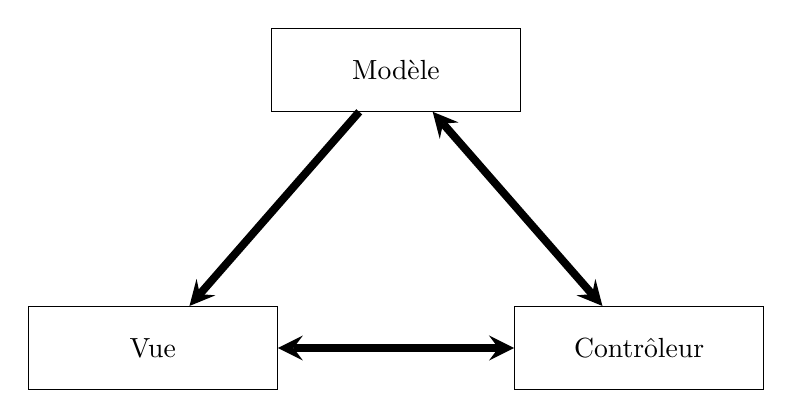
\begin{tikzpicture}[
      elementblock/.style={draw,rectangle,minimum height=3em, minimum width=9em},
      node distance=3cm]
    % Blocks
    \node[elementblock]                                     (view)      {Vue};
    \node[elementblock,right=of view]                       (controller){Contr\^oleur};
    \node[elementblock,above=of {$(view)!0.5!(controller)$}](model)     {Mod\`ele};

    % Arrows
    \draw[         -{stealth},thick,line width=0.1cm] (model) edge (view);
    \draw[{stealth}-{stealth},thick,line width=0.1cm] (model) edge (controller) (controller) edge (view);

  \end{tikzpicture}
  \caption{Mod\`ele-Vue-Contr\^oleur}
\end{figure}
% ======================================================

Les contr\^oleurs sont plac\'es dans le package \texttt{runtime}, les mod\`eles dans le package \texttt{game\_mechanics} et les vues dans le package \texttt{gui}.

\section{Les contr\^oleurs}

Le contr\^oleur principal est l'objet \texttt{Controller}. Il contient la boucle \texttt{update}-\texttt{render} ainsi que l'ensemble des mod\`eles actifs : les tours, les ennemis et les projectiles. \`A chaque tour de boucle, tous ces mod\`eles sont mis \`a jour et dessin\'es \`a l'\'ecran. La mise \`a jour des mouvements se fait par m\'ethode d'Euler (plus de d\'etails en section \ref{models}).

% Needs more stuff in here :)

\section{Mod\`eles} \label{models}

% TODO

\section{Vues}

% TODO

\section{Conclusion} % Maybe ?

% TODO

\end{document}
